\documentclass[conference]{IEEEtran}
\IEEEoverridecommandlockouts
\usepackage{cite}
\usepackage{amsmath,amssymb,amsfonts}
\usepackage{graphicx}
\graphicspath{{figures/}}
\usepackage{textcomp}
\usepackage{xcolor}
\usepackage{booktabs}
\usepackage[obeyspaces]{url}
\usepackage{multirow}
\usepackage{hyperref}
\usepackage{tikz}
\usetikzlibrary{positioning, arrows.meta, calc}
\usepackage{tabularx}
\usepackage[margin=1in]{geometry}
\usepackage{forest}
\usepackage{color}  
\usepackage{stfloats}

\forestset{
  mynode/.style={draw, rounded corners, font=\small, align=center, inner sep=2pt},
  root/.style={mynode, fill=gray!20, font=\bfseries},
  L1/.style={mynode, fill=blue!15},
  L2/.style={mynode, fill=white, draw=black!60},
  leaf/.style={font=\scriptsize, align=left, text width=2.8cm, inner sep=1pt},
  edge/.style={-{Stealth[length=2.5pt]}, thick},
} 

\def\BibTeX{{\rm B\kern-.05em{\sc i\kern-.025em b}\kern-.08em
    T\kern-.1667em\lower.7ex\hbox{E}\kern-.125emX}}  


\begin{document}

\title{A Systematic Literature Review of I/O Stack Evolution for Fully Utilizing SSDs}

\author{\IEEEauthorblockN{Dawen Liang}
\IEEEauthorblockA{\textit{College of Engineering and Computer Science}\\
\textit{Syracuse University}\\
Syracuse, NY, USA\\
dliang02@hotmail.com}
\and
\IEEEauthorblockN{Hengbo Cai}
\IEEEauthorblockA{\textit{College of Engineering and Computer Science}\\
\textit{Syracuse University}\\
Syracuse, NY, USA\\
chb59468@hotmail.com}
}

\maketitle

\begin{abstract}
The rise of ultra-low latency (ULL) NVMe SSDs, which have device access times nearing single-digit microseconds, has drastically changed the performance bottleneck from storage hardware to the software I/O stack. This systematic literature review examines how the I/O stack has evolved---from kernel-based mediation to hybrid and full kernel bypass solutions---to fully harness the capabilities of modern SSDs. Following PRISMA 2020 guidelines~\cite{page2021prisma}, we gathered 3{,}131 records from four databases and via citation-based snowballing, eventually including 398 studies covering the period from 2012--2025. We organize the reviewed work into a three-path taxonomy: \emph{Kernel Path} optimizations (multi-queue block layer, io\_uring, polling, and file system adaptations), \emph{Hybrid Approaches} (eBPF/XRP in-kernel bypass, NVMe I/O Passthrough, and modernized FUSE), and \emph{Full Kernel Bypass} solutions (SPDK, user-space file systems, and interrupt-based user-space stacks). Key findings include: (1)~the Linux kernel storage path contributes up to 50\% of end-to-end I/O latency when using modern NVMe devices; (2)~promising optimizations in the kernel path, like blk-switch, achieve an average latency improvement of up to $130\times$ over standard Linux; (3)~hybrid approaches such as XRP and I/O Passthru deliver throughput gains of 30--94\% while maintaining kernel safety guarantees; and (4)~full bypass platforms continue to advance beyond SPDK toward energy-efficient and interrupt-based designs. We identify convergence trends---particularly the blurring of kernel and bypass boundaries through eBPF programmability and NVMe passthrough---and outline open challenges including multi-tenancy, security, and energy efficiency for upcoming I/O stack research.
\end{abstract}

\begin{IEEEkeywords}
I/O stack, block layer, ultra-low latency SSD, NVMe, kernel bypass, io\_uring, SPDK, eBPF, systematic literature review
\end{IEEEkeywords}

\section{Introduction}
\label{sec:intro}

The performance of solid-state drives (SSDs) has seen significant improvements over the last decade. Modern NVMe SSDs offer random read latencies below 10\,$\mu$s and sequential bandwidths above 7\,GB/s, approaching the throughput limits of the PCIe interconnect~\cite{koh2018exploring, lee2022nvmectrl}. This rapid hardware advancement challenges a long-held assumption in systems design: for ultra-low latency (ULL) SSDs, the \emph{software} I/O stack---not the storage device---has become the dominant performance bottleneck.

Barroso et al. identified this paradigm shift as the ``attack of the killer microseconds,'' observing that neither nanosecond-scale hardware techniques (branch prediction, prefetching) nor millisecond-scale software techniques (context switching, thread-based concurrency) are effective for microsecond-regime operations~\cite{barroso2017killer}. Enberg et al. further demonstrated that hardware queue constraints in modern processors (e.g., at most 10 Line Fill Buffers per core) impose fundamental limits on prefetch-based latency hiding, while application-managed queues incur management overhead that caps peak performance at 50\% of the DRAM baseline~\cite{enberg2017taming}.

The traditional Linux I/O stack---comprising the Virtual File System (VFS), file system, page cache, block layer, and device driver---was designed when storage devices operated at millisecond latencies~\cite{io2021faster}. Fig.~\ref{fig:iostack} illustrates this layered architecture, where each I/O request traverses the system call interface, file system, block layer (with blk-mq per-core queues), and device driver before reaching the hardware~\cite{hwang2021rearchitecting, zhang2018flashshare, liu2022towards}. With ULL SSDs, these software layers introduce overheads that were previously negligible: context switches, data copies between kernel and user buffers, interrupt handling, I/O scheduling, and lock contention.

\begin{figure}[t]
\centering
\hspace{-2mm}
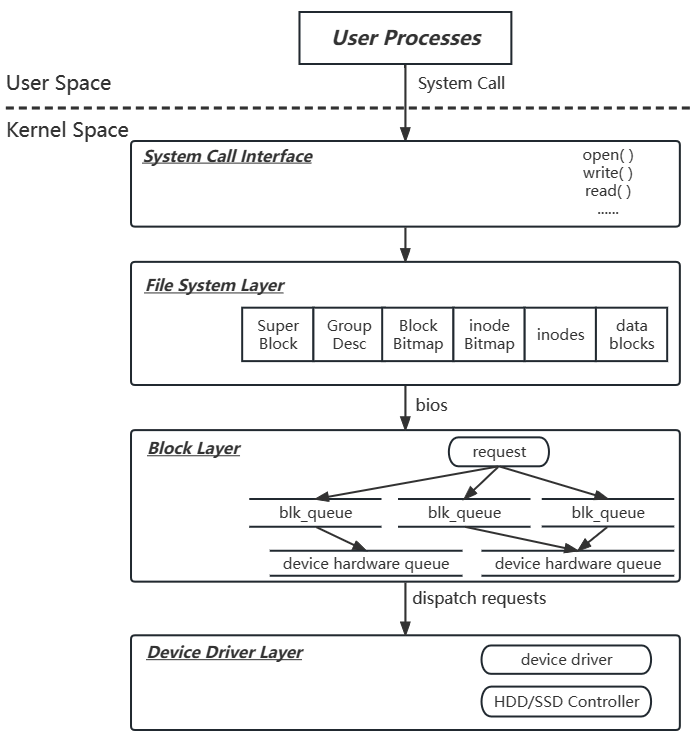
\includegraphics[width=1.00\columnwidth]{fig_iostack.png}
\caption{The traditional Linux I/O stack. Each I/O request from user space traverses multiple kernel layers---system call interface, file system, block layer (with blk-mq per-core queues), and device driver---before reaching the storage device~\cite{hwang2021rearchitecting, zhang2018flashshare, liu2022towards}.}
\label{fig:iostack}
\end{figure}

The asynchronous I/O stack by Lee et al. demonstrated that overlapping kernel operations with device I/O can reduce full-path latency to below 10\,$\mu$s for 4\,KB random reads on Intel Optane SSDs---a 15--33\% improvement over the traditional path~\cite{lee2019asynchronous}. Yet even with such optimizations, the kernel's contribution to end-to-end latency remains substantial. As Fig.~\ref{fig:scm} illustrates, Storage Class Memory (SCM) devices such as Intel Optane, Samsung Z-SSD, and KIOXIA XL-Flash bridge the latency gap between DRAM ($\sim$100\,ns) and conventional NVMe SSDs (150--250\,$\mu$s) with access times around 15\,$\mu$s, further exacerbating the software overhead problem. Fig.~\ref{fig:latency} confirms this quantitatively: for ULL devices such as Z-SSD and Optane, the kernel accounts for 24--36\% of total I/O latency, while for 4\,KB random writes with \texttt{fsync}, kernel overhead reaches 29--36\% even on NVMe SSDs~\cite{liu2022towards}.

\begin{figure}[t]
\centering
\hspace{-2mm}
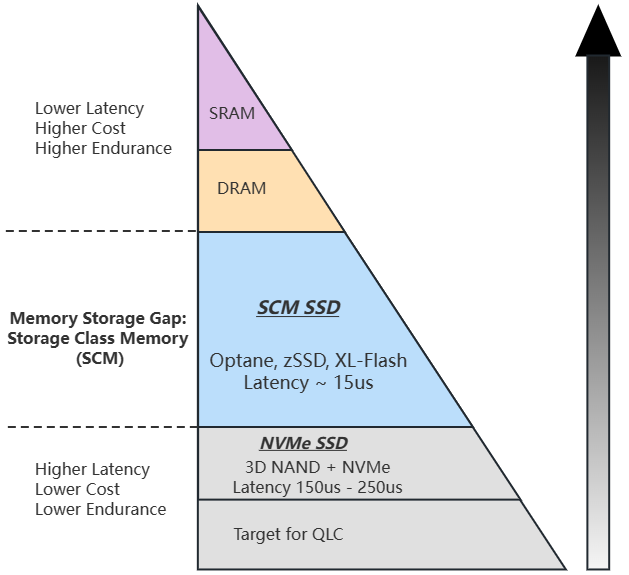
\includegraphics[width=1.00\columnwidth]{fig_scm_hierarchy.png}
\caption{Storage Class Memory (SCM) in the memory--storage hierarchy. SCM SSDs (Optane, Z-SSD, XL-Flash) with $\sim$15\,$\mu$s latency bridge the gap between DRAM and conventional NVMe SSDs, making software I/O stack overhead the dominant bottleneck.}
\label{fig:scm}
\end{figure}

\begin{figure*}[t]
\centering
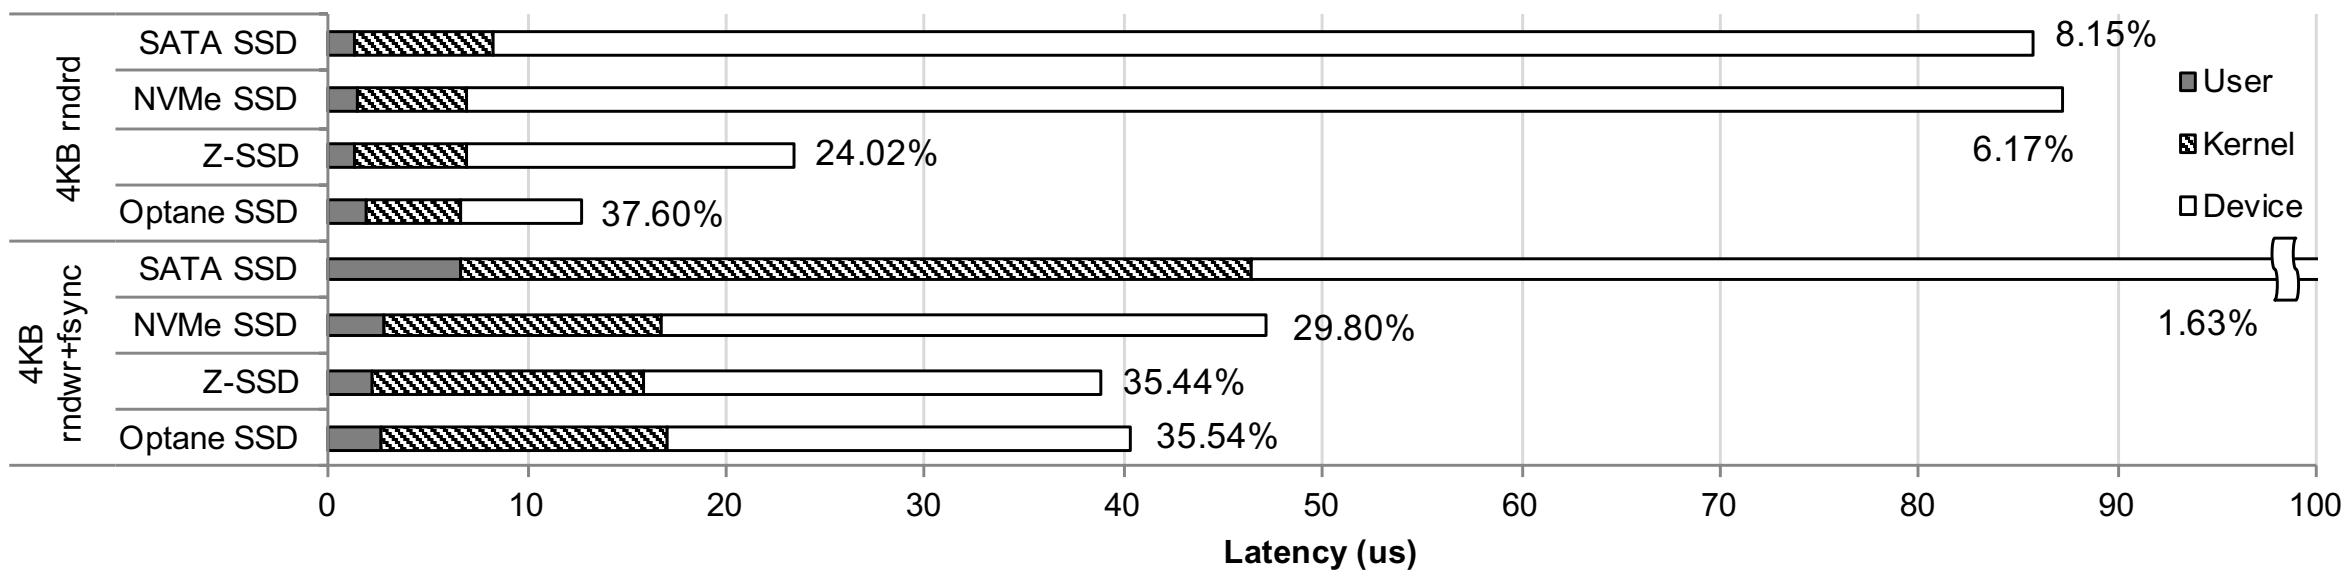
\includegraphics[width=\textwidth]{fig_latency_breakdown.png}
\caption{I/O latency breakdown across storage devices. Percentages indicate the kernel's share of total latency. As device speed increases from SATA SSD to Optane SSD, the kernel's relative contribution grows from 8\% to 38\% for 4\,KB random reads. Source: adapted from~\cite{liu2022towards}.}
\label{fig:latency}
\end{figure*}

In response, the research community has explored three broad architectural strategies. \emph{Kernel path optimizations} retain the existing Linux I/O architecture but reduce overhead through multi-queue block layers (blk-mq)~\cite{bjorling2013linux}, advanced scheduling~\cite{lee2021d2fq}, and asynchronous interfaces (io\_uring)~\cite{didona2022understanding}. \emph{Hybrid approaches} selectively bypass specific kernel layers while preserving others, exemplified by eBPF-based storage functions (XRP)~\cite{zhong2022xrp}, NVMe I/O Passthrough~\cite{joshi2024iopassthru}, and modernized user-space file system frameworks (RFUSE)~\cite{rfuse2024}. \emph{Full kernel bypass} solutions remove the kernel entirely from the data path, led by Intel's SPDK~\cite{yang2017spdk} and user-space file systems such as uFS~\cite{liu2021scale} and NVMeDirect~\cite{kim2016user}.

Despite this rich body of work, no existing survey systematically covers the full spectrum of I/O stack evolution from 2012 to 2025 using a reproducible methodology. Prior surveys have addressed specific aspects---Didona et al.~\cite{didona2022understanding} compared storage APIs, and Koh et al.~\cite{koh2018exploring} characterized ULL SSD performance---but a comprehensive, PRISMA-compliant review spanning kernel, hybrid, and bypass approaches is lacking.

This paper addresses that gap. We conducted a systematic literature review following PRISMA 2020 guidelines~\cite{page2021prisma}, identifying 398 relevant studies from a pool of 3{,}131 records. Our contributions are:
\begin{itemize}
\item A reproducible, PRISMA-compliant search and screening methodology across four databases plus snowballing, yielding a corpus of 398 included studies with quality assessment.
\item A three-path taxonomy (Kernel, Hybrid, Full Bypass) that organizes the surveyed work and reveals convergence trends.
\item A technical synthesis of 44 deeply analyzed papers covering innovations from blk-mq (2013) to interrupt-based user-space stacks (2025).
\item Identification of open challenges and future directions for I/O stack research in the era of sub-microsecond storage.
\end{itemize}

The remainder of this paper is organized as follows. Section~\ref{sec:method} describes our research methodology. Section~\ref{sec:results} presents the search and screening results. Section~\ref{sec:survey} provides the technical survey organized by the three-path taxonomy. Section~\ref{sec:discussion} discusses cross-cutting themes and implications. Section~\ref{sec:future} outlines future research directions, and Section~\ref{sec:conclusion} concludes.


%% ============================================================
\section{Research Methodology}
\label{sec:method}
%% ============================================================

We performed a systematic literature review in line with PRISMA 2020 guidelines~\cite{page2021prisma}. Our methodology encompasses five phases: formulating research questions, conducting a systematic search, two-stage screening, quality assessment, and data extraction. This review covers research published between 2012 and May 2025.

\subsection{Research Questions}

Drawing on the PICOC framework (Population: ULL NVMe SSDs; Intervention: I/O stack software optimization; Comparison: traditional Linux block layer / POSIX I/O; Outcomes: latency, throughput, CPU efficiency; Context: OS kernel and system software), we formulated four research questions:

\begin{itemize}
\item \textbf{RQ1:} How have I/O stack design principles changed from traditional HDD-based systems to modern SSD-focused solutions?
\item \textbf{RQ2:} Which traditional I/O stack principles are still valid for ULL SSDs, and how have they been modified?
\item \textbf{RQ3:} What new principles and methods have appeared to meet the performance and scalability needs of ULL SSDs?
\item \textbf{RQ4:} What future research directions and challenges must be confronted to further optimize I/O stacks for high-performance storage?
\end{itemize}

\subsection{Search Strategy}

We searched four electronic databases and supplemented with citation-based snowballing (Table~\ref{tab:sources}). Five Boolean query strings were created to cover the main I/O stack optimization technologies (Table~\ref{tab:queries}). Each query was executed against DB1--DB4 with the search cutoff set to May 31, 2025. For DB5, we performed forward and backward citation tracing on six seed papers, including seminal works on SPDK~\cite{yang2017spdk}, the asynchronous I/O stack~\cite{lee2019asynchronous}, and FlashShare~\cite{zhang2018flashshare}.

Additionally, 80 papers from the first author's prior review work were included as a supplementary source. These papers had been independently curated through an earlier search process and entered the current review at the full-text assessment stage (Stage~2), where they were subjected to the same eligibility criteria as database-sourced records.

\begin{table}[t]
\caption{Search Sources}
\label{tab:sources}
\centering
\small
\begin{tabular}{@{}lll@{}}
\toprule
ID & Source & Type \\
\midrule
DB1 & Google Scholar & General academic \\
DB2 & ACM Digital Library & CS-specific \\
DB3 & IEEE Xplore & CS/EE-specific \\
DB4 & Semantic Scholar (API) & Multidisciplinary \\
DB5 & Forward/backward snowballing & Citation tracing \\
\bottomrule
\end{tabular}
\end{table}

\begin{table}[t]
\caption{Query Strings}
\label{tab:queries}
\centering
\small
\begin{tabular}{@{}cp{5.5cm}@{}}
\toprule
QID & Query String \\
\midrule
Q1 & ``io\_uring'' OR ``SPDK'' OR ``blk-mq'' NVMe SSD performance \\
Q2 & ``kernel bypass'' NVMe storage latency \\
Q3 & eBPF storage ``I/O stack'' OR ``storage stack'' NVMe \\
Q4 & ``ultra-low latency'' SSD ``I/O'' optimization kernel \\
Q5 & NVMe ``user-space'' OR ``userspace'' driver file system \\
\bottomrule
\end{tabular}
\end{table}

\subsection{Inclusion and Exclusion Criteria}

Studies were included if they: (a)~examine I/O stack software optimizations aimed at NVMe or ULL SSDs; (b)~present designs, implementations, or evaluations of kernel-path, hybrid, or full kernel-bypass I/O approaches; or (c)~provide empirical performance data in the context of modern SSD storage.

Exclusion was governed by five mutually exclusive criteria applied in strict priority order (EC1~$>$~EC2~$>$~EC3~$>$~EC4~$>$~EC5):

\begin{table}[t]
\caption{Exclusion Criteria}
\label{tab:exclusion}
\centering
\small
\begin{tabular}{@{}cl@{}}
\toprule
Code & Definition \\
\midrule
EC1 & Non-computer-science domain \\
EC2 & Pure hardware (no software stack contribution) \\
EC3 & Not focused on ULL I/O stack optimization \\
EC4 & Non-peer-reviewed (with critical exceptions) \\
EC5 & Duplicate contribution (superseded version) \\
\bottomrule
\end{tabular}
\end{table}

\noindent
\textbf{Scope boundary:} Research on CXL (Compute Express Link), ZNS-only optimizations lacking contributions to the I/O stack, KV-SSD interfaces, and computational storage offloading was excluded under EC3.

\subsection{Screening Process}

After combining records from all sources, 710 duplicates were identified by DOI match and normalized title similarity, leaving 2{,}341 unique records.

\textbf{Stage~1} (title and abstract screening) excluded 1{,}849 records: EC1:~39, EC2:~18, EC3:~1{,}677, EC4:~115. The high number of EC3 exclusions reflects a broad search strategy aimed at maximum recall.

\textbf{Stage~2} (full-text eligibility) assessed 572 reports (492 from Stage~1 plus 80 prior-review papers) and excluded 174: EC1:~105, EC2:~17, EC3:~48, EC4:~2, EC5:~2. The final included corpus comprises \textbf{398 studies}.

The arithmetic checksum verifies: $398 + 174 + 1{,}849 + 710 = 3{,}131$.

\subsection{Quality Assessment}

Each included study was scored on a 0--3 quality scale:

\begin{table}[t]
\caption{Quality Assessment Distribution}
\label{tab:qa}
\centering
\small
\begin{tabularx}{\columnwidth}{c X c c X}
\toprule
Score & Criteria & Count & \% & Role \\
\midrule
3 & Top-tier venue + artifacts & 72 & 18.1 & Primary evidence \\
2 & Recognized venue + solid eval & 65 & 16.3 & Supporting \\
1 & \url{Workshop/short/limited eval} & 52 & 13.1 & Supplementary \\
0 & Minimal evaluation & 209 & 52.5 & Audit only \\
\bottomrule
\end{tabularx}
\end{table}

The 209 studies scored QA\,=\,0 remain in the included count for audit transparency but are excluded from the technical synthesis. Sections~\ref{sec:survey} and~\ref{sec:discussion} draw exclusively from the 189 studies scoring QA\,$\geq$\,1.

\subsection{Data Extraction and Classification}

For each study, we gathered bibliographic metadata, Path\_Type classification (\emph{Kernel}, \emph{Hybrid}, or \emph{Full Bypass}), key technologies used, optimization techniques, and reported performance metrics. The Path\_Type taxonomy serves as the main organizational structure for Section~\ref{sec:survey}.

%% ============================================================
\section{Search Results}
\label{sec:results}
%% ============================================================

This section reports the outcome of the systematic search and screening process and presents descriptive statistics of the included corpus.

\subsection{PRISMA Flow}

A total of 3{,}131 records were identified: 3{,}051 from database searches (DB1--DB5) and 80 from the first author's prior review work. After removing 710 duplicates, 2{,}341 unique records entered Stage~1 screening. Title and abstract screening excluded 1{,}849 records, with most of these (1{,}677; 90.7\% of Stage~1 exclusions) removed under EC3. The remaining 492 records were combined with the 80 prior-review papers for Stage~2 full-text assessment, during which 174 reports were excluded. The final included corpus comprises 398 studies (Fig.~\ref{fig:prisma}).

\begin{figure*}[t]
\centering
\resizebox{\textwidth}{!}{%
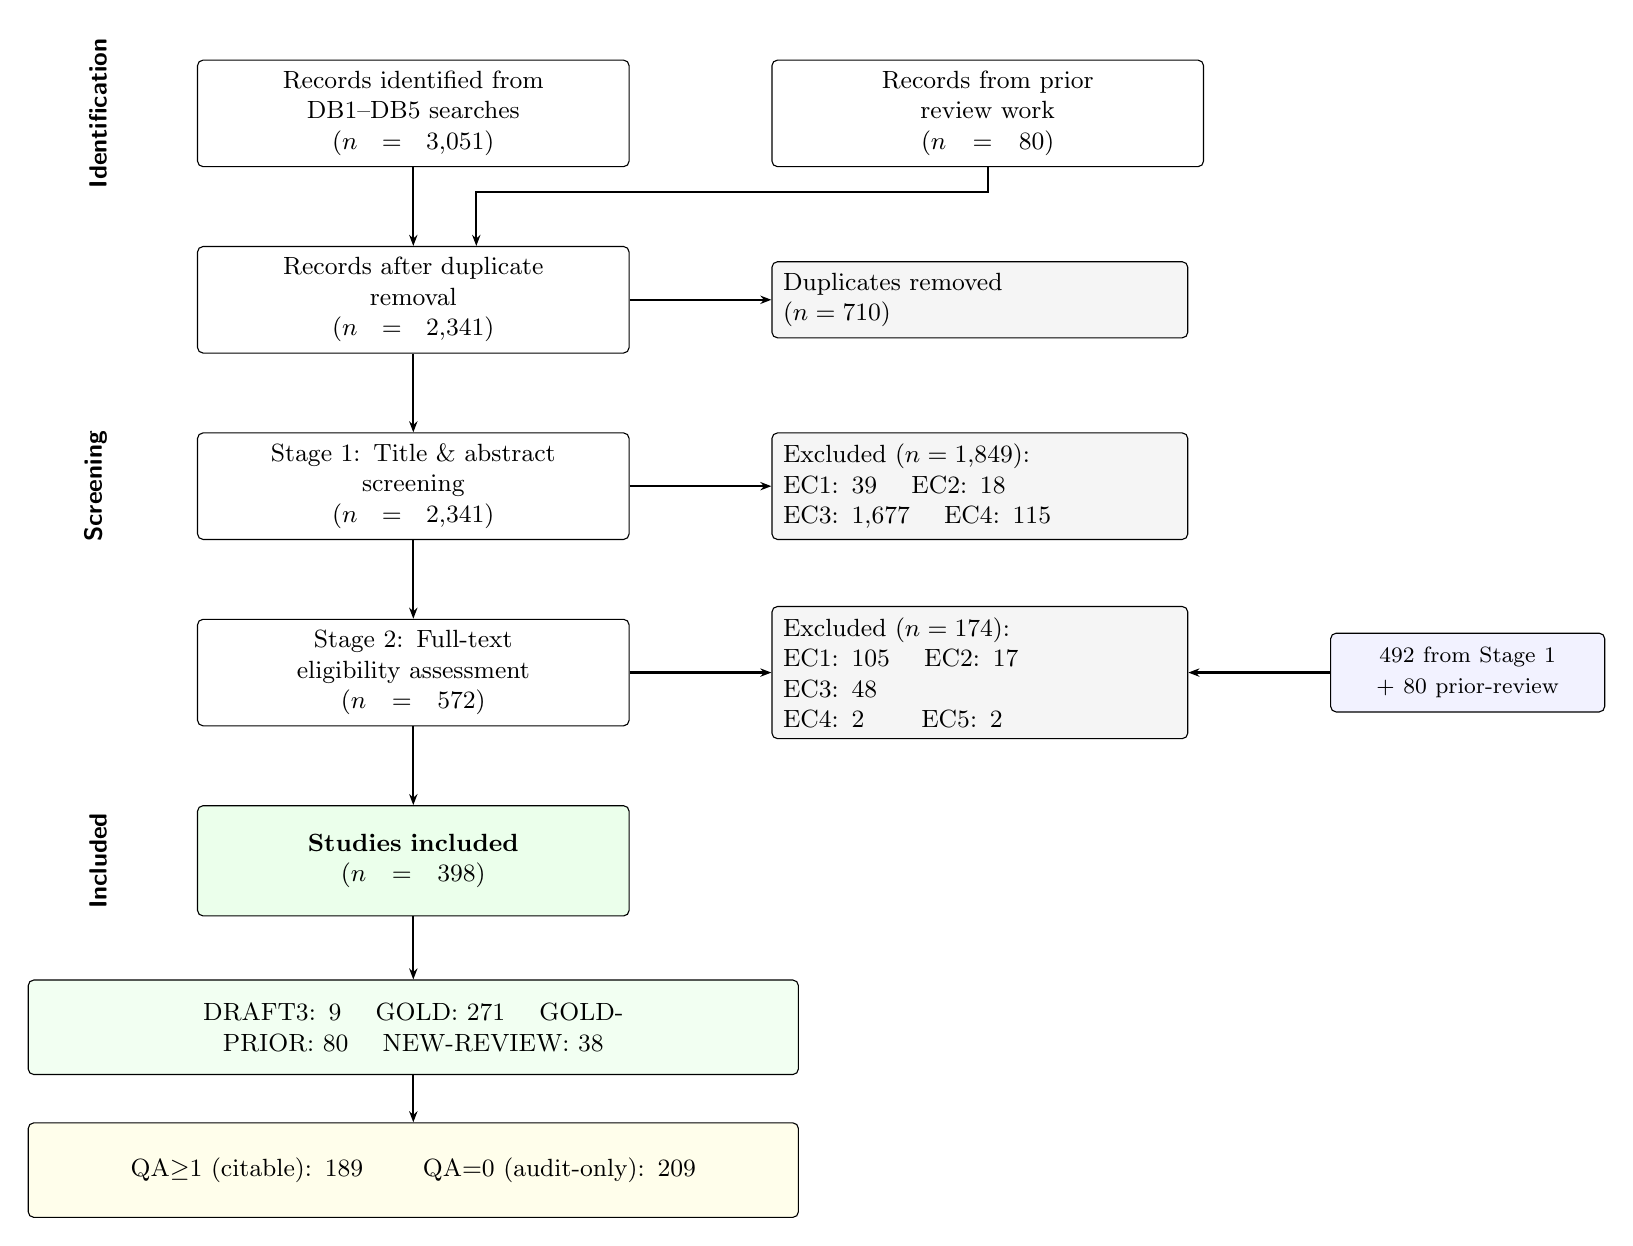
\begin{tikzpicture}[
  box/.style={draw, rounded corners=2pt, text width=#1, minimum height=10mm, align=center, font=\small},
  box/.default=42mm,
  excl/.style={draw, rounded corners=2pt, text width=50mm, align=left, font=\small, fill=gray!8},
  phase/.style={font=\small\bfseries\sffamily, rotate=90, anchor=south},
  arr/.style={-{Stealth[length=4pt]}, thick},
  every node/.style={inner sep=4pt},
]

% === IDENTIFICATION ===
\node[box=52mm] (id_db) {Records identified from\\DB1--DB5 searches\\($n = 3{,}051$)};
\node[box=52mm, right=18mm of id_db] (id_other) {Records from prior\\review work\\($n = 80$)};

% Phase label
\node[phase, left=10mm of id_db.west, anchor=south, yshift=0mm] {\textsf{Identification}};

% === DEDUP ===
\node[box=52mm, below=10mm of id_db] (dedup) {Records after duplicate\\removal\\($n = 2{,}341$)};
\node[excl, right=18mm of dedup] (dup_excl) {Duplicates removed\\($n = 710$)};

\draw[arr] (id_db) -- (dedup);
\draw[arr] (id_other) -- ++(0,-10mm) -| ([xshift=8mm]dedup.north);
\draw[arr] (dedup) -- (dup_excl);

% === STAGE 1 SCREENING ===
\node[box=52mm, below=10mm of dedup] (s1) {Stage~1: Title \& abstract\\screening\\($n = 2{,}341$)};
\node[excl, right=18mm of s1] (s1_excl) {Excluded ($n = 1{,}849$):\\EC1: 39 \quad EC2: 18\\EC3: 1{,}677 \quad EC4: 115};

% Phase label
\node[phase, left=10mm of s1.west, anchor=south, yshift=0mm] {\textsf{Screening}};

\draw[arr] (dedup) -- (s1);
\draw[arr] (s1) -- (s1_excl);

% === STAGE 2 ELIGIBILITY ===
\node[box=52mm, below=10mm of s1] (s2) {Stage~2: Full-text\\eligibility assessment\\($n = 572$)};
\node[excl, right=18mm of s2] (s2_excl) {Excluded ($n = 174$):\\EC1: 105 \quad EC2: 17\\EC3: 48\\ EC4: 2 \quad\;\; EC5: 2};

\node[box=32mm, right=18mm of s2_excl, fill=blue!5] (prior_note) {\footnotesize 492 from Stage~1\\+ 80 prior-review};

\draw[arr] (s1) -- (s2);
\draw[arr] (s2) -- (s2_excl);
\draw[arr] (prior_note) -- (s2_excl);

% === INCLUDED ===
\node[box=52mm, below=10mm of s2, fill=green!8, minimum height=14mm] (incl) {\textbf{Studies included}\\($n = 398$)};

% Phase label
\node[phase, left=10mm of incl.west, anchor=south, yshift=0mm] {\textsf{Included}};

\draw[arr] (s2) -- (incl);

% === BREAKDOWN ===
\node[box=95mm, below=8mm of incl, fill=green!5, minimum height=12mm] (breakdown) {DRAFT3: 9 \quad GOLD: 271 \quad GOLD-PRIOR: 80 \quad NEW-REVIEW: 38};

\draw[arr] (incl) -- (breakdown);

% === QA ===
\node[box=95mm, below=6mm of breakdown, fill=yellow!8, minimum height=12mm] (qa) {QA$\geq$1 (citable): 189 \qquad QA$=$0 (audit-only): 209};

\draw[arr] (breakdown) -- (qa);

\end{tikzpicture}
}%
\caption{PRISMA 2020 flow diagram. EC1--EC5 denote the exclusion criteria defined in Table~\ref{tab:exclusion}. The 80 prior-review papers enter at Stage~2 after independent confirmation. The arithmetic checksum verifies: $398 + 174 + 1{,}849 + 710 = 3{,}131$.}
\label{fig:prisma}
\end{figure*}

\subsection{Publication Year Distribution}

The corpus spans over a decade of I/O stack research, with a clear increase in publication volume from 2019 onward. The 2012--2015 period (16 papers, 4.0\%) includes foundational work like blk-mq and early polling studies. The 2016--2018 period (50 papers, 12.6\%) saw the growth of NVMeDirect, FlashShare, and SPDK. The most productive period is 2019--2021 (74 papers, 18.6\%), which includes the debut of io\_uring, the asynchronous I/O stack, and XRP. The 2022--2025 period (135 papers, 33.9\%) introduced significant designs such as I/O Passthru, RFUSE, BypassD, and Aeolia. An additional 123 papers (30.9\%) from curated collections lack complete year metadata.

\subsection{Venue Distribution}

Among the 240 papers with identifiable venue metadata, USENIX venues (FAST, ATC, OSDI, HotStorage) account for 47 papers, reflecting the systems research community's sustained focus on optimizing the storage stack. Conference proceedings dominate (153 papers), followed by journal articles (54), preprints (11), and other venues (22).

\subsection{Source Category Breakdown}

The 398 included studies consist of: DRAFT3 (9 seed papers hand-selected for the initial manuscript), GOLD (271 papers from the author's curated collection independently confirmed by DB1--DB5), GOLD-PRIOR (80 papers from prior work not captured by current searches), and NEW-REVIEW (38 newly discovered 2024--2025 papers). The GOLD category (68.1\%) shows significant overlap between the systematic search and prior work, providing confidence in search recall.


%% ============================================================
\section{Technical Survey of I/O Stack Evolution (2013--2025)}
\label{sec:survey}
%% ============================================================


\begin{figure*}[!t]
\centering
\resizebox{0.9\textwidth}{!}{%
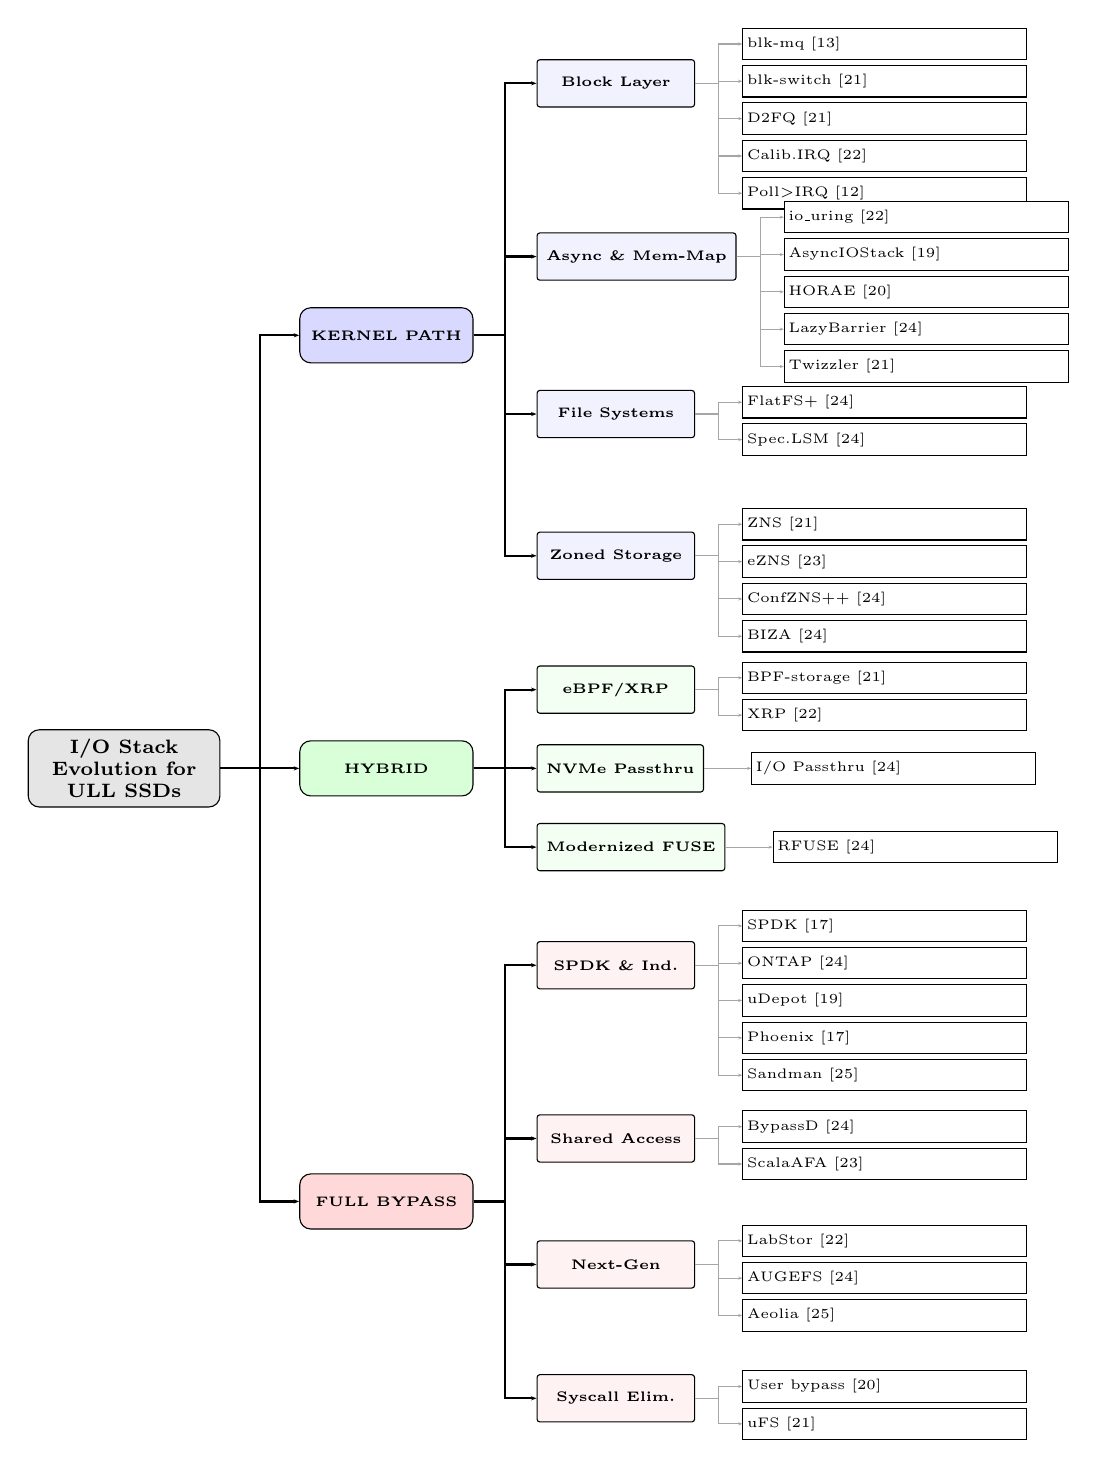
\begin{tikzpicture}[
  root/.style={draw, rounded corners, fill=gray!20, font=\bfseries\scriptsize, text width=22mm, align=center, minimum height=8mm},
  L1/.style={draw, rounded corners, font=\bfseries\tiny, minimum width=22mm, minimum height=7mm, inner sep=2pt},
  L2/.style={draw, rounded corners=1pt, font=\bfseries\tiny, minimum width=20mm, minimum height=6mm, fill=white},
  leaf/.style={draw, thin, fill=white, font=\tiny, anchor=west, text width=35mm, inner sep=1.5pt, minimum height=4mm},
  arr/.style={-{Stealth[length=2pt]}, thick},
  line/.style={draw, -{Stealth[length=1.5pt]}, thin, gray!70},
]

% --- Root node ---
\node[root] (root) at (0,0) {I/O Stack\\Evolution for\\ULL SSDs};

% --- Level 1 ---
\node[L1, fill=blue!15, right=10mm of root, yshift=55mm] (kern) {KERNEL PATH};
\node[L1, fill=green!15, right=10mm of root, yshift=0mm] (hyb) {HYBRID};
\node[L1, fill=red!15, right=10mm of root, yshift=-55mm] (byp) {FULL BYPASS};

\draw[arr] (root.east) -- ++(5mm,0) |- (kern.west);
\draw[arr] (root.east) -- (hyb.west);
\draw[arr] (root.east) -- ++(5mm,0) |- (byp.west);

% --- Level 2: KERNEL ---
\node[L2, fill=blue!5, right=8mm of kern, yshift=32mm] (blk) {Block Layer};
\node[L2, fill=blue!5, right=8mm of kern, yshift=10mm] (aio) {Async \& Mem-Map};
\node[L2, fill=blue!5, right=8mm of kern, yshift=-10mm] (fs) {File Systems};
\node[L2, fill=blue!5, right=8mm of kern, yshift=-28mm] (zns) {Zoned Storage};

\foreach \sub in {blk, aio, fs, zns} { \draw[arr] (kern.east) -- ++(4mm,0) |- (\sub.west); }

% KERNEL leaves
\node[leaf] (k1) at ([xshift=6mm, yshift=5mm]blk.east) {blk-mq [13]};
\node[leaf] (k2) [below=0.6mm of k1] {blk-switch [21]};
\node[leaf] (k3) [below=0.6mm of k2] {D2FQ [21]};
\node[leaf] (k4) [below=0.6mm of k3] {Calib.IRQ [22]};
\node[leaf] (k5) [below=0.6mm of k4] {Poll$>$IRQ [12]};
\foreach \p in {k1,k2,k3,k4,k5} { \draw[line] (blk.east) -- ++(3mm,0) |- (\p.west); }

\node[leaf] (k6) at ([xshift=6mm, yshift=5mm]aio.east) {io\_uring [22]};
\node[leaf] (k7) [below=0.6mm of k6] {AsyncIOStack [19]};
\node[leaf] (k8) [below=0.6mm of k7] {HORAE [20]};
\node[leaf] (k9) [below=0.6mm of k8] {LazyBarrier [24]};
\node[leaf] (k10) [below=0.6mm of k9] {Twizzler [21]};
\foreach \p in {k6,k7,k8,k9,k10} { \draw[line] (aio.east) -- ++(3mm,0) |- (\p.west); }

\node[leaf] (k11) at ([xshift=6mm, yshift=1.5mm]fs.east) {FlatFS+ [24]};
\node[leaf] (k12) [below=0.6mm of k11] {Spec.LSM [24]};
\foreach \p in {k11,k12} { \draw[line] (fs.east) -- ++(3mm,0) |- (\p.west); }

\node[leaf] (k13) at ([xshift=6mm, yshift=4mm]zns.east) {ZNS [21]};
\node[leaf] (k14) [below=0.6mm of k13] {eZNS [23]};
\node[leaf] (k15) [below=0.6mm of k14] {ConfZNS++ [24]};
\node[leaf] (k16) [below=0.6mm of k15] {BIZA [24]};
\foreach \p in {k13,k14,k15,k16} { \draw[line] (zns.east) -- ++(3mm,0) |- (\p.west); }

% --- Level 2: HYBRID ---
\node[L2, fill=green!5, right=8mm of hyb, yshift=10mm] (ebpf) {eBPF/XRP};
\node[L2, fill=green!5, right=8mm of hyb, yshift=0mm] (pass) {NVMe Passthru};
\node[L2, fill=green!5, right=8mm of hyb, yshift=-10mm] (fuse) {Modernized FUSE};

\foreach \sub in {ebpf, pass, fuse} { \draw[arr] (hyb.east) -- ++(4mm,0) |- (\sub.west); }

\node[leaf] (h1) at ([xshift=6mm, yshift=1.5mm]ebpf.east) {BPF-storage [21]};
\node[leaf] (h2) [below=0.6mm of h1] {XRP [22]};
\foreach \p in {h1,h2} { \draw[line] (ebpf.east) -- ++(3mm,0) |- (\p.west); }

\node[leaf] (h3) at ([xshift=6mm]pass.east) {I/O Passthru [24]};
\draw[line] (pass.east) -- ++(3mm,0) -- (h3.west);

\node[leaf] (h4) at ([xshift=6mm]fuse.east) {RFUSE [24]};
\draw[line] (fuse.east) -- ++(3mm,0) -- (h4.west);

% --- Level 2: FULL BYPASS ---
\node[L2, fill=red!5, right=8mm of byp, yshift=30mm] (spdk) {SPDK \& Ind.};
\node[L2, fill=red!5, right=8mm of byp, yshift=8mm] (shared) {Shared Access};
\node[L2, fill=red!5, right=8mm of byp, yshift=-8mm] (nextg) {Next-Gen};
\node[L2, fill=red!5, right=8mm of byp, yshift=-25mm] (sysc) {Syscall Elim.};

\foreach \sub in {spdk, shared, nextg, sysc} { \draw[arr] (byp.east) -- ++(4mm,0) |- (\sub.west); }

\node[leaf] (b1) at ([xshift=6mm, yshift=5mm]spdk.east) {SPDK [17]};
\node[leaf] (b2) [below=0.6mm of b1] {ONTAP [24]};
\node[leaf] (b3) [below=0.6mm of b2] {uDepot [19]};
\node[leaf] (b4) [below=0.6mm of b3] {Phoenix [17]};
\node[leaf] (b5) [below=0.6mm of b4] {Sandman [25]};
\foreach \p in {b1,b2,b3,b4,b5} { \draw[line] (spdk.east) -- ++(3mm,0) |- (\p.west); }

\node[leaf] (b6) at ([xshift=6mm, yshift=1.5mm]shared.east) {BypassD [24]};
\node[leaf] (b7) [below=0.6mm of b6] {ScalaAFA [23]};
\foreach \p in {b6,b7} { \draw[line] (shared.east) -- ++(3mm,0) |- (\p.west); }

\node[leaf] (b8) at ([xshift=6mm, yshift=3mm]nextg.east) {LabStor [22]};
\node[leaf] (b9) [below=0.6mm of b8] {AUGEFS [24]};
\node[leaf] (b10) [below=0.6mm of b9] {Aeolia [25]};
\foreach \p in {b8,b9,b10} { \draw[line] (nextg.east) -- ++(3mm,0) |- (\p.west); }

\node[leaf] (b11) at ([xshift=6mm, yshift=1.5mm]sysc.east) {User bypass [20]};
\node[leaf] (b12) [below=0.6mm of b11] {uFS [21]};
\foreach \p in {b11,b12} { \draw[line] (sysc.east) -- ++(3mm,0) |- (\p.west); }

\end{tikzpicture}
}%
\caption{Taxonomy of I/O stack optimization approaches for ULL SSDs. The 44 deeply analyzed works are organized along three architectural paths: Kernel Path (optimizations within the existing Linux I/O stack), Hybrid (selective layer bypass), and Full Bypass (complete kernel removal from the data path). Year labels indicate publication date.}
\label{fig:taxonomy}
\end{figure*}

This section synthesizes the technical contributions of 44 deeply analyzed papers, organized along the three-path taxonomy shown in Fig.~\ref{fig:taxonomy}: Kernel Path optimizations (\S\ref{sec:kernel}), Hybrid Approaches (\S\ref{sec:hybrid}), and Full Kernel Bypass (\S\ref{sec:bypass}). We also discuss cross-cutting concerns (\S\ref{sec:crosscut}) that span multiple paths.

%% ------------------------------------------------------------
\subsection{Kernel Path Optimizations}
\label{sec:kernel}
%% ------------------------------------------------------------

Kernel path optimizations keep the Linux I/O stack architecture but systematically reduce overhead at each layer. We group these into four areas: block layer improvements, asynchronous and memory-mapped I/O, file system changes, and zoned storage interfaces.

\subsubsection{Block Layer: Multi-Queue and Scheduling}
\label{sec:blkmq}

The introduction of the multi-queue block layer (blk-mq) by Bj{\o}rling et al.\ in 2013 marked a foundational change~\cite{bjorling2013linux}. It replaced the single-queue block layer with per-core software queues that map to hardware submission and completion queues in NVMe devices. This design removed a major bottleneck and allowed the block layer to scale with modern multi-core, multi-queue hardware.

Despite improvements from blk-mq, head-of-line blocking between latency-sensitive and throughput-oriented requests remained a critical issue in multi-tenant environments. Hwang et al.\ tackled this with blk-switch~\cite{hwang2021rearchitecting}, which applies network switch design principles to the storage stack. The key insight is that Linux's per-core block layer queues, alongside multi-queue hardware, make the storage stack similar to a multi-ingress, multi-egress network switch. blk-switch uses this similarity to implement request-level and thread-level load balancing across cores, achieving up to $130\times$ better average latency and $24\times$ better P99 latency over baseline Linux while maintaining 84--100\% of throughput. Notably, blk-switch also outperforms SPDK in tail latency by up to $12\times$ and $18\times$ for average and P99 latency, respectively, showing that kernel-path methods can compete with full bypass in mixed workloads.

I/O scheduling overhead has also been examined for ULL devices. Lee et al.\ proposed D2FQ (Device-Direct Fair Queueing), which combines I/O submission and dispatch into a single step by using the NVMe Weighted Round Robin (WRR) arbitration mechanism on the device side~\cite{lee2021d2fq}. D2FQ saves up to 45\% of CPU cycles compared to the latest MQFQ scheduler while reducing I/O latency by 35\% and increasing bandwidth by 54\%. This device-direct approach finds an important middle ground between traditional kernel scheduling and complete kernel bypass, allowing scheduling decisions to be made by the device hardware itself.

Harris and Altiparmak evaluated whether I/O schedulers are still beneficial for ULL devices~\cite{sched2021needed}. Their findings are clear: for ULL storage, schedulers like mq-deadline and kyber add 0.5--0.9\,$\mu$s (around 6\%) to median latency, while bfq can increase it by up to 2.5\,$\mu$s (20\%). They concluded that I/O schedulers have become unnecessary for ULL devices when the focus is on performance or energy efficiency. However, they acknowledge that schedulers can be valuable for fairness and quality of service on slower devices.

The I/O completion mechanism---interrupts versus polling---represents another important optimization area. Yang et al.\ first demonstrated in 2012 that polling is better than interrupt-driven I/O for emerging fast storage devices~\cite{yang2012poll}. This insight lays the groundwork for much of the later I/O stack optimization work. Building on this, Yang et al.\ proposed calibrated interrupts, a hybrid approach where applications explicitly mark latency-sensitive requests using a minimal two-bit device interface change~\cite{yang2022calibrated}. The device adjusts its interrupt timing to match the completion of latency-sensitive requests, achieving up to 35\% higher throughput, 30\% lower CPU use, and 37\% lower latency compared to traditional coalesced interrupts.

Harris and Altiparmak also showed that classic polling on ULL devices can be more energy-efficient than interrupts, contrary to common belief~\cite{wang2022pollvsenergy}. They found that CPU use does not directly correlate with overall system power consumption. With a single thread, classic polling achieves 8.1\,$\mu$s latency (2\,$\mu$s better than interrupts) with no context switches.

\begin{figure}[t]
\centering
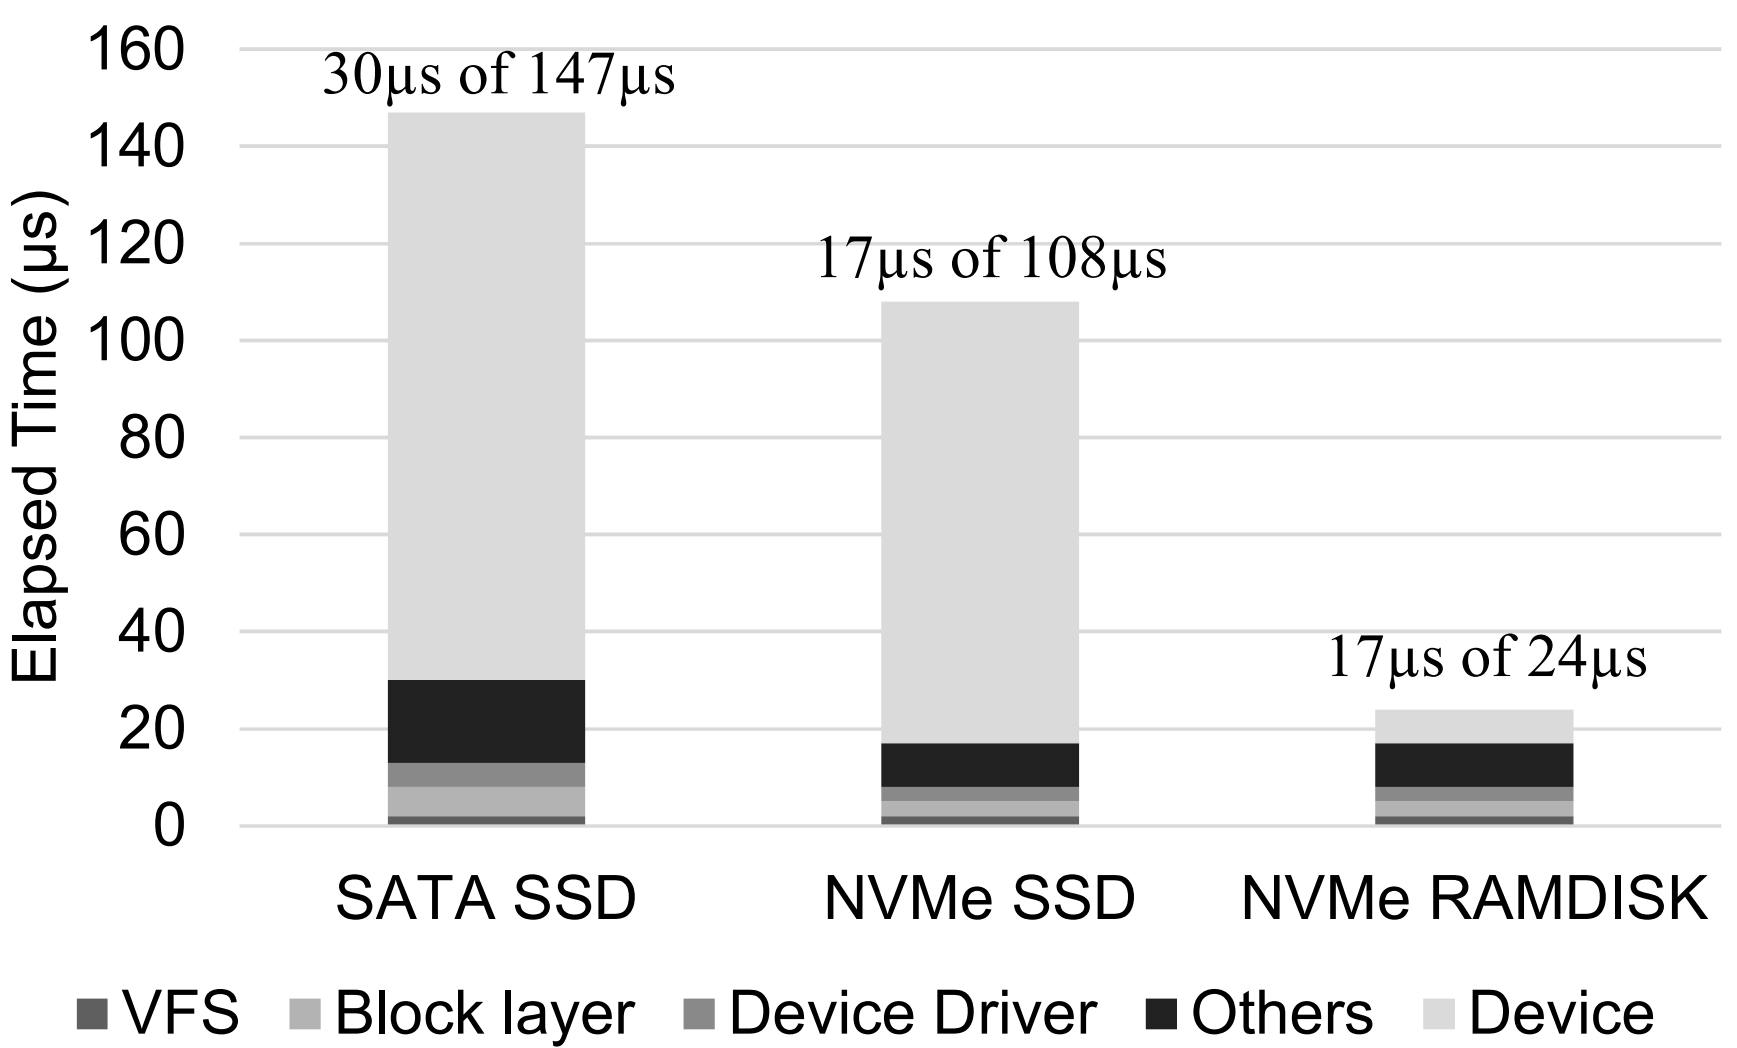
\includegraphics[width=0.85\columnwidth]{fig_elapsed_time.png}
\caption{Comparison of elapsed time per I/O stack layer across SATA SSD, NVMe SSD, and NVMe RAMDISK. Software overhead (VFS + Block layer + Device Driver) is 30\,$\mu$s of 147\,$\mu$s total for SATA, but 17\,$\mu$s of 24\,$\mu$s (71\%) for NVMe RAMDISK, demonstrating that software becomes the dominant bottleneck as device latency decreases. Source: adapted from~\cite{kim2017framework}.}
\label{fig:elapsed}
\end{figure}

\subsubsection{Asynchronous and Memory-Mapped I/O}
\label{sec:async}

The io\_uring interface, introduced in Linux 5.1, offers a high-performance asynchronous I/O option through shared submission and completion queues between user space and the kernel. This avoids the overhead of per-request system calls. Didona et al.~\cite{didona2022understanding} systematically compared io\_uring against SPDK and libaio, concluding that io\_uring can reach SPDK-level performance when properly configured with polling modes. However, it requires careful tuning and attention to CPU resource use.

The asynchronous I/O stack by Lee et al.~\cite{lee2019asynchronous} showed that specific operations within the kernel read and write paths---extent tree preloading, asynchronous page allocation, lazy page cache indexing, and lazy DMA unmapping---can overlap with device time. Combined with a lightweight block I/O layer that eliminates merging and scheduling delays, this approach achieved latencies below 10\,$\mu$s for 4\,KB random reads on Optane SSDs.

Write ordering constraints add more overhead in the kernel path. Liang et al.\ introduced HORAE~\cite{liang2020horae}, which separates the control of write dependencies from the data flow by using MMIO for ordering control and the standard block layer for data flow. This architectural change avoids combining multiple hardware queues into a single logical queue, which can lead to overhead as high as 87\% with increasing queue counts. HORAE delivers performance improvements of up to $1.8\times$ and $2.1\times$ in MySQL and BlueStore, respectively.

LazyBarrier~\cite{lazybarrier2024} addresses barrier write overhead in the Android I/O stack, where \texttt{fsync()} achieves only 3.9\% of buffered write throughput. Its ``Lazy Issue'' mechanism shares global and greedy barrier write command (BWC) across threads, paired with per-hardware-queue FIFO scheduling. This results in 73\% higher throughput than the no-barrier baseline (dual-thread) and reduces latency from 51\,$\mu$s to 20\,$\mu$s. This shows that smart kernel algorithms can yield significant improvements without needing kernel bypass.

Memory-mapped I/O has also been re-examined for fast storage. Papagiannis et al.~\cite{papagiannis2020mmap} identified scaling issues in the Linux mmap path for quick devices and proposed optimizations such as reducing TLB shootdowns and handling page faults in parallel. Twizzler~\cite{peter2021twizzler} takes a bolder approach, suggesting a ``data-centric'' operating system where persistent data is accessed through memory-mapped objects with persistent pointers. This eliminates the traditional process-centric model and its related I/O stack overhead entirely.

\subsubsection{File System Adaptations}
\label{sec:fs}

Managing file system metadata can be a challenge when storage systems operate with microsecond latencies. Son et al.\ proposed FlatFS+~\cite{son2024flatns}, which replaces traditional hierarchical namespaces with a flat namespace architecture tailored for byte-addressable NVMs. This change reduces the overhead linked to metadata lookups that can slow down fast storage.

Wu et al.\ tackled the access path of KV-stores using speculative multi-level access in LSM tree-based stores~\cite{park2022speculative}. Their method switches from synchronous I/O to asynchronous I/O for reading data blocks, allowing multiple SSTables to be accessed at the same time. With 16 client threads, their solution boosts throughput by up to 85\% compared to baseline RocksDB, although it results in 9--26\% over-fetched I/O requests, showing the tradeoff between performance and resources common in asynchronous optimization.

UnistorFS~\cite{wu2020unistorfs} presents a union storage file system that removes the line between memory and storage on PRAM devices. It allows interchangeable page management using a new \texttt{GFP\_UNISTOR} flag in the Linux kernel's allocation system. This method cuts down on unnecessary data movement and improves resource use by enabling memory and storage pages to function together without logical partitioning.

\subsubsection{Zoned Storage Interfaces}
\label{sec:zns}

The Zoned Namespace (ZNS) interface reconsiders the host--device relationship. Bj{\o}rling et al.~\cite{bjorling2021zns} showed that the traditional block interface carries a significant ``tax'' for flash SSDs due to capacity over-provisioning, DRAM for page mapping tables, and garbage collection overhead. ZNS SSDs can deliver up to $2.7\times$ higher throughput than block-interface SSDs in concurrent write tasks and up to 64\% lower average random read latency. Using RocksDB on f2fs/ZNS results in $2$--$4\times$ lower P99.9 read tail latency.

Several studies have built on ZNS to address its drawbacks. Han et al.\ introduced ZNS+~\cite{han2021znsplus}, which adds in-storage zone compaction to cut down on write amplification and reduce CPU overhead on the host. LightNVM~\cite{bjorling2017lightnvm} previously led the way in developing the open-channel SSD subsystem in Linux, advocating that SSD management choices should be handled by host software rather than hidden firmware.

Lee et al.\ presented eZNS~\cite{lee2023ezns}, an elastic zoned namespace that tackles the limitations of fixed zone setups. eZNS incorporates zone ballooning, which adjusts zone stripe widths based on workload needs, a hardware abstraction layer that requires only three device parameters, and a smart read scheduler. This strategy draws from virtualization memory ballooning to improve resource use among co-located namespaces.

ConfZNS++~\cite{park2024confznspp} highlights that even host-controlled interfaces like ZNS can introduce new kinds of I/O management interference. The study shows that host-issued I/O management tasks, such as zone resets or finishes, interfere with data I/O. It proposes two solutions: ZINC, an I/O scheduler that prioritizes data I/O over management tasks (reducing reset interference by 56.9\%), and a soft-finish operation (reducing finish interference by 50.7\%).

BIZA~\cite{chen2024biza} closes the compatibility gap between block interfaces and ZNS by combining a block-to-ZNS adapter with RAIZN into one unified layer. BIZA addresses the issue that current I/O stacks do not guarantee the order in which requests are submitted---a single in-flight write can lose up to 65.3\% throughput with ZNS. Through intra-zone parallelism via the Zone Random Write Area (ZRWA) and coordinated garbage collection across layers, BIZA lowers write amplification by 42.7\%, boosts write throughput by 93.2\%, and cuts P99.99 tail latency by 62.8\%.

ZMS~\cite{zms2024} expands zone abstractions to mobile flash storage (UFS, not NVMe), achieving $5.0$--$13.6\times$ better random write performance and $2.9$--$6.4\times$ lower write amplification through cross-layer optimization involving the file system, block layer, and firmware.

%% ------------------------------------------------------------
\subsection{Hybrid Approaches}
\label{sec:hybrid}
%% ------------------------------------------------------------

Hybrid methods selectively bypass certain kernel layers while keeping others in place, creating a design space between full kernel mediation and complete bypassing. This area has seen vibrant development from 2021 to 2025, fueled by eBPF programmability, NVMe passthrough, and modern user-space frameworks.

\subsubsection{eBPF/XRP: In-Kernel Bypass}
\label{sec:xrp}

The idea that eBPF can serve as a basis for storage optimization was first described by Zhong et al.\ in their HotOS position paper~\cite{bpf2021storage}. They indicated that the kernel storage path contributes to about half of the access latency in modern NVMe devices. An analysis of software overhead shows that ext4 accounts for 32.0\%, the BIO layer for 6.0\%, and kernel crossings for 8.8\%.

This concept was put into practice with XRP~\cite{zhong2022xrp}, which allows applications to run user-defined storage functions (like index lookups and aggregations) from an eBPF hook in the NVMe driver, securely bypassing most of the kernel's storage stack. Unlike complete kernel bypass, eBPF is an OS-supported tool that ensures isolation and avoids the low utilization that busy-waiting can cause. For dependent I/O chains, which are common in B-tree lookups, XRP achieves 47--94\% higher throughput and 20--34\% lower P99 latency than using \texttt{read()}. XRP also facilitates better core sharing than SPDK, showing a 56\% improvement in P99 latency when two threads share the same core.

To maintain file system principles, XRP forwards a small amount of kernel state (file extent mappings) to the NVMe driver hook using a soft-state cache that takes advantage of the relative stability of file extents. This design ensures the safety of the file system while allowing for application-specific tweaks at a strategic point in the I/O stack.

\subsubsection{NVMe Passthrough (I/O Passthru)}
\label{sec:passthru}

Joshi et al.~\cite{joshi2024iopassthru} introduced I/O Passthru, a new I/O path in Linux that skips the block layer entirely using a character-device interface (\texttt{/dev/ng0n1}) along with \texttt{io\_uring\_cmd}. The key motivation goes beyond just performance. The block interface cannot represent all NVMe features, including ZNS with non-power-of-two zone sizes, extended LBA formats, and KV command sets. I/O Passthru reaches 5M IOPS, which is 31\% higher than the 3.83M IOPS of the block path, with a handler latency of only 144\,ns compared to 209\,ns for the block path. This method has been integrated into the Linux kernel from versions 5.13 to 6.2, representing a production-ready hybrid solution.

In practical deployments, I/O Passthru supports Flexible Data Placement (FDP), reducing write amplification from $>$2 to approximately~1.

\subsubsection{Modernized FUSE (RFUSE)}
\label{sec:rfuse}

The traditional FUSE framework struggles with significant performance issues due to its single shared pending queue, which creates lock contention and prevents user-space file systems from performing well. RFUSE~\cite{rfuse2024} modernizes FUSE with three main improvements: per-core ring channels that replace the shared pending queue, hybrid polling (50\,$\mu$s busy-wait then sleep), and improved path traversal. RFUSE achieves 53\% lower latency and $2.27\times$ higher throughput compared to FUSE for random reads, coming close to EXT4 performance in macro-benchmarks while maintaining full API compatibility with existing FUSE file systems. This success shows that traditional systems can be updated to achieve competitive performance instead of being discarded.

\subsubsection{BPF for Storage: The Exokernel Vision}
\label{sec:bpf}

Zhong et al.'s earlier position paper~\cite{bpf2021storage} outlined a broader vision for BPF in storage, inspired by exokernel file systems. The paper suggested triggering BPF functions in the NVMe driver interrupt handler for each block I/O completion. This gives those functions access to raw block buffers to determine file offsets and quickly reissue any dependent I/O tasks. This approach has led to throughput improvements of up to $2.5\times$ and latency reductions of 49\% for dependent I/O chains.

A significant design challenge is maintaining file system safety guarantees, especially with address translation between physical blocks and file offsets. The authors address this by caching extent metadata at the NVMe layer.

%% ------------------------------------------------------------
\subsection{Full Kernel Bypass}
\label{sec:bypass}
%% ------------------------------------------------------------

Full kernel bypass removes the kernel completely from the data-path I/O. This change allows user-space applications to interact directly with NVMe devices. SPDK~\cite{yang2017spdk} remains the leading framework. However, recent efforts address its key limitations: device sharing, energy efficiency, modularity, and the polling assumption.

\subsubsection{SPDK and Industrial Adoption}
\label{sec:spdk}

SPDK offers user-space NVMe drivers, polled-mode application scheduling (one thread per core with lockless queues), and implementations for storage protocols. SPDK achieves around 7\,$\mu$s read latency and 8\,$\mu$s write latency for 4\,KB random I/O at queue depth~1. This results in a 44\% reduction in latency for reads and a 36\% reduction for writes compared to the kernel stack~\cite{yang2017spdk}.

The industrial impact of SPDK-based architectures is shown by ONTAP's evolution~\cite{curtismaury2024ontap}. NetApp's ONTAP storage system, which was originally designed for spinning drives, underwent years of optimization for SSDs. The main strategy included layer bypassing: WAFL Reply Fastpath removed message-passing hops between software components, and RAID Fastpath bypassed the RAID component on the read path. These improvements cut software overhead from multiple milliseconds to under 160\,$\mu$s (more than $20\times$), increasing read throughput at an average latency of 1\,ms. ONTAP's experience confirms that incremental layer bypassing for error-free data paths is an effective and safe optimization strategy for production systems.

uDepot~\cite{kourtis2019udepot} showcases the practical use of user-space I/O principles for KV stores. It is built on the TRT (Task Runtime for Taming) framework with both libaio and SPDK backends. uDepot achieves $1.95$--$2.1\times$ better YCSB throughput compared to Aerospike and $10.2$--$14.7\times$ better than ScyllaDB, demonstrating the benefits of kernel bypass, polling instead of interrupts, and minimal cross-core communication.

Phoenix~\cite{li2017phoenix} uses memory-centric I/O interfaces for HPC workloads. It models all I/O as operations on persistent memory objects and takes advantage of aggregate DRAM+NVM bandwidth. This approach leads to up to $12\times$ performance improvement through a redesign of the I/O stack.

Sandman~\cite{zhou2025sandman} addresses SPDK's biggest practical limitation: 100\% CPU utilization from busy-polling. It uses hardware user wait instructions (\texttt{monitorx}/\texttt{mwaitx}) for microsecond-level workload detection and shallow C-1 sleep. Sandman reduces power consumption by 39.38\% and energy use by 33.36\% while staying within 5\% of SPDK's peak performance. This method was validated against Alibaba and Tencent field traces, making it suitable for cloud deployments.

\subsubsection{Shared Access and Scalability}
\label{sec:shared}

Device sharing remains a key challenge for kernel bypass. If each application needs exclusive NVMe queue access, multi-tenant setups become impractical. Kim et al.\ tackled this with BypassD~\cite{yadalam2024bypassd}. It implements a split architecture where latency-critical data operations (\texttt{read()}, \texttt{write()}) run directly in user space, while metadata operations (\texttt{open()}, appends) are handled by the kernel. BypassD suggests IOMMU improvements to translate virtual block addresses (VBAs) for hardware-enforced isolation between tenants, without kernel mediation on the data path.

ScalaAFA~\cite{lee2023scalaafa} addresses the scalability of user-space all-flash array engines. Based on SPDK's lock-free approach, ScalaAFA replaces traditional locks with message-passing for permission management. It uses SSD-internal compute resources for parity computation during RAID conversion. ScalaAFA achieves $2.5\times$ the write throughput and 52.7\% lower average write latency compared to the best AFA engines available.

\subsubsection{Next-Generation Bypass Platforms}
\label{sec:nextgen}

LabStor~\cite{lukken2022labstor} introduces a modular, extensible platform for building customized I/O stacks in user space. The core abstraction is the \emph{LabMod}, an independent code module that provides single-purpose storage functionality. These modules can be swapped, stacked, and hot-upgraded. LabStor's modular design addresses three main issues of Linux file systems: performance degradation from workload-agnostic policies, significant software overhead from context switching and data copying, and limited flexibility due to POSIX compliance. Performance tests show the SPDK LabMod outperforming POSIX by up to 60\% for 4\,KB I/Os.

AUGEFS~\cite{kim2024augefs} develops a scalable user-space log-structured file system. It includes three main innovations: a shared and protected address space that ensures library-level file system performance with cross-process sharing; METADB, an LSM-tree-based metadata store that removes false sharing through parallel request processing; and domain-based file organization for independent space management and parallel operations. AUGEFS also introduces an asynchronous I/O stack for \texttt{fsync} that allows data block and node block I/O to overlap, which reduces synchronous write latency.

The most radical shift in conventional bypass designs is Aeolia~\cite{zhou2025aeolia}. It challenges the widely accepted idea that polling is necessary for high-performance user-space storage. Aeolia shows that most overhead previously linked to interrupts actually comes from kernel thread scheduling policies, not the interrupts themselves. By integrating user-space interrupts with MPK (hardware intra-process isolation) and \texttt{sched\_ext} (eBPF-based scheduling), Aeolia creates an interrupt-based user-space storage stack that occupies a new area in the design landscape. AeoDriver outperforms io\_uring with polling and SPDK by $8.18\times$ to $291.72\times$ when running latency-critical and compute-heavy tasks, because event-driven interrupt handling prevents CPU wastage due to polling and the issues of concurrent programming based on polling.

\subsubsection{Syscall Elimination}
\label{sec:syscall}

Park and Volos~\cite{park2020bypass} introduced userspace bypass (UB), which moves user-space instructions into the kernel to remove system call overhead. With KPTI enabled, a single no-op system call costs 431 CPU cycles, and a \texttt{pwrite} can lower subsequent instruction IPC from 2.9 to 0.2. UB achieves 30.3--88.3\% acceleration for I/O micro-benchmarks without needing any changes to application code. While it may be less effective than io\_uring or DPDK for specific workloads, UB's requirement for zero modifications offers a distinct advantage in the design landscape.

uFS~\cite{liu2021scale} creates a user-level file system semi-microkernel based on SPDK. The uFS server carefully separates in-memory data structures and on-disk data at the inode level. This design achieves share-nothing semantics between worker threads connected to client applications through lockless ring buffers. This architecture results in a flexible, scalable, and high-performance user-space file system with POSIX-style APIs.

%% ------------------------------------------------------------
\subsection{Cross-Cutting Concerns}
\label{sec:crosscut}
%% ------------------------------------------------------------

Several themes appear across the kernel, hybrid, and bypass paths, highlighting key challenges in designing I/O stacks for ULL SSDs.

\subsubsection{The Killer Microsecond Problem}
\label{sec:killer}

Barroso et al.~\cite{barroso2017killer} identified microsecond operations as lying in a ``no man's land'' between fast hardware techniques and slower software techniques. Software delays, acceptable for HDDs---such as a cumulative 75\,$\mu$s from RPC and TCP/IP stacks on a 2\,$\mu$s fabric---become the main latency issue for ULL devices.

Enberg et al.~\cite{enberg2017taming} quantified hardware limits: Line Fill Buffers restrict prefetches to 10 per core, and a shared on-chip interconnect queue (capacity 14) creates a bottleneck for multicore systems. Application-managed queues can get around the LFB limit but come with management costs that cap performance at 50\% of the DRAM baseline.

The ``I/O is faster than the CPU'' position~\cite{io2021faster} argues that many OS abstractions, designed when I/O was slower than the CPU, are now outdated. It suggests a ``parakernel'' architecture that allocates hardware queues per process. This theoretical idea drives practical efforts across all three I/O paths.

\subsubsection{Zero-Copy and Data Movement Optimization}
\label{sec:zerocopy}

Data copying between kernel and user buffers takes up 10--35\% of total I/O latency with modern SSDs~\cite{kim2022zerocopy}. Kim et al.\ proposed a hybrid zero-copy I/O stack that checks the page cache during buffered reads: cache hits go through normally, while cache misses trigger direct transfers from the device to the user buffer, bypassing the kernel buffer completely. Delayed prefetching selectively refills the cache, minimizing conflicts with current I/O. This method cuts latency by up to 25\% and boosts throughput by up to 27\%.

Kim and Lee~\cite{kim2021zero} further examined balancing data validity (which needs cache coherence) with zero-copy (bypassing the cache). Their strategy delays cache filling by reading directly into user buffers on cache misses and fills the cache asynchronously when conditions allow.

\subsubsection{Latency Characterization and Hardware Acceleration}
\label{sec:latchar}

Liu et al.~\cite{liu2022towards} provided a detailed analysis of I/O latency across SATA SSDs, NVMe SSDs, Z-SSDs, and Optane devices. They found that kernel overhead rises from 8\% to 36\% of total latency as device speed increases (Fig.~\ref{fig:latency}). Their work on mixed-workload I/O services for ULL SSDs highlighted the need for scheduling that considers workloads.

Lee et al.~\cite{lee2022nvmectrl} introduced a high-performance NVMe controller with hardware acceleration, reaching 7.0\,GB/s bandwidth and 1.7M IOPS, with average latencies of only 2.4\,$\mu$s (read) and 3.2\,$\mu$s (write), using 89\% of PCIe bandwidth. This co-design approach shifts intensive data transfer tasks to hardware while keeping complex commands in firmware.

Since NVMe firmware can make up 86--99\% of total I/O latency in PRAM and MRAM devices, hardware acceleration at the controller level offers a way to complement optimizations on the host side. FLIXR~\cite{he2022flixr} shows cross-stack optimization by incorporating index data into FTL entries, removing the need for separate index I/O operations. With SSD controller processors idle for almost 70\% of the time even under high I/O loads, FLIXR takes advantage of this slack to improve performance by 52.6\% for TPC-C/TPC-H benchmarks with minimal changes to firmware.

\subsubsection{Virtualized and Cloud Storage}
\label{sec:virt}

Spool~\cite{min2021spool} addresses reliability issues in virtualized NVMe storage pools, pointing out that SPDK's initialization process takes about 2.5\,s to probe all devices and set up the Environment Abstraction Layer. During software updates, all I/O devices become unavailable, which is disruptive for cloud storage. Spool presents live-upgradable virtualized storage pools that keep I/O available during system maintenance.

Choi et al.~\cite{choi2019managing} show that with NVMe SSDs delivering 5\,GB/s read and 3\,GB/s write speeds (which exceed 10/25GbE networks), the network has become the real bottleneck for SSD arrays, not the storage itself. Their sequential management method, which allows only one SSD to handle write requests at a time, fundamentally rethinks storage array design as individual devices are no longer the limiting factor.

%% ============================================================
\section{Discussion}
\label{sec:discussion}
%% ============================================================


\begin{figure*}[t]
\centering
\resizebox{\textwidth}{!}{%
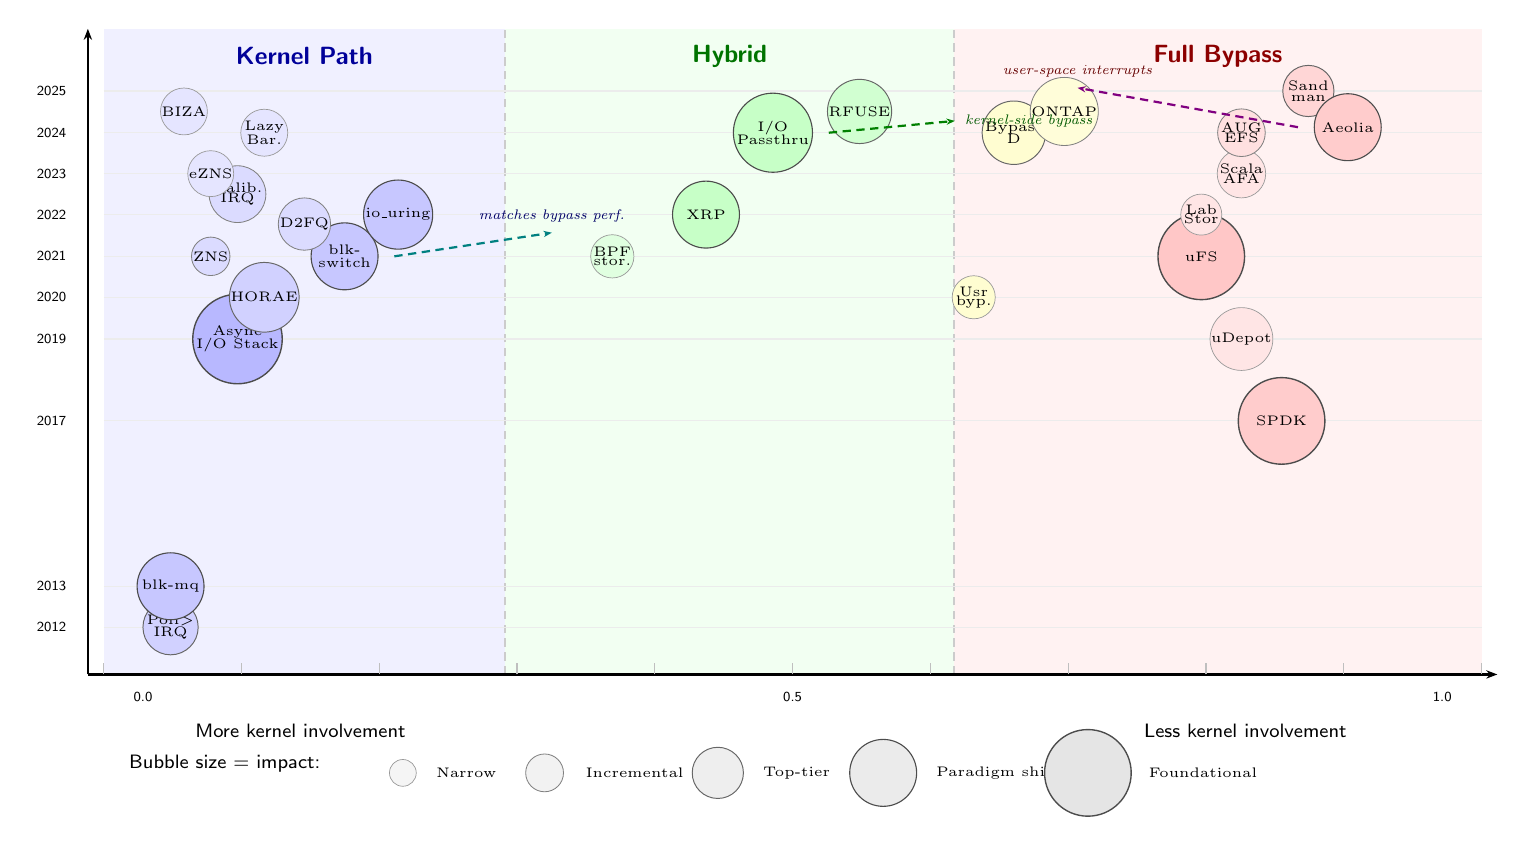
\begin{tikzpicture}[
  % Bubble styles — 5 levels
  b5/.style={circle, draw=black!70, line width=0.5pt, minimum size=11mm, font=\fontsize{4.8}{5.4}\selectfont, align=center, inner sep=0.5pt},
  b4/.style={circle, draw=black!70, line width=0.4pt, minimum size=8.5mm, font=\fontsize{4.3}{5}\selectfont, align=center, inner sep=0.5pt},
  b3/.style={circle, draw=black!60, line width=0.35pt, minimum size=6.5mm, font=\fontsize{4}{4.6}\selectfont, align=center, inner sep=0.3pt},
  b2/.style={circle, draw=black!50, line width=0.3pt, minimum size=4.8mm, font=\fontsize{3.6}{4.2}\selectfont, align=center, inner sep=0.3pt},
  b1/.style={circle, draw=black!40, line width=0.25pt, minimum size=3.4mm, font=\fontsize{3.2}{3.8}\selectfont, align=center, inner sep=0.2pt},
  conv/.style={-{Stealth[length=3pt]}, densely dashed, thick},
]

% Background zones
\fill[blue!6] (0, -0.6) rectangle (5.1, 7.6);
\fill[green!5] (5.1, -0.6) rectangle (10.8, 7.6);
\fill[red!5] (10.8, -0.6) rectangle (17.5, 7.6);

% Zone dividers
\draw[gray!40, densely dashed, line width=0.6pt] (5.1, -0.6) -- (5.1, 7.6);
\draw[gray!40, densely dashed, line width=0.6pt] (10.8, -0.6) -- (10.8, 7.6);

% Zone labels
\node[font=\small\bfseries\sffamily, blue!60!black] at (2.55, 7.25) {Kernel Path};
\node[font=\small\bfseries\sffamily, green!45!black] at (7.95, 7.25) {Hybrid};
\node[font=\small\bfseries\sffamily, red!55!black] at (14.15, 7.25) {Full Bypass};

% X-axis
\draw[-{Stealth[length=4pt]}, thick] (-0.2, -0.6) -- (17.7, -0.6);
\node[font=\tiny\sffamily, anchor=north] at (0.5, -0.7) {0.0};
\node[font=\tiny\sffamily, anchor=north] at (8.75, -0.7) {0.5};
\node[font=\tiny\sffamily, anchor=north] at (17.0, -0.7) {1.0};
\node[font=\scriptsize\sffamily, anchor=north] at (2.5, -1.1) {More kernel involvement};
\node[font=\scriptsize\sffamily, anchor=north] at (14.5, -1.1) {Less kernel involvement};
\foreach \v in {0,1.75,3.5,5.25,7.0,8.75,10.5,12.25,14.0,15.75,17.5} {
  \draw[gray!50] (\v, -0.6) -- (\v, -0.45);
}

% Y-axis (year)
\draw[-{Stealth[length=4pt]}, thick] (-0.2, -0.6) -- (-0.2, 7.6);
\foreach \yr/\ypos in {2012/0, 2013/0.52, 2017/2.62, 2019/3.66, 2020/4.19, 2021/4.71, 2022/5.24, 2023/5.76, 2024/6.28, 2025/6.81} {
  \node[font=\tiny\sffamily, anchor=east] at (-0.35, \ypos) {\yr};
  \draw[gray!15] (0, \ypos) -- (17.5, \ypos);
}

% ========== KERNEL PATH (blue) ==========

% Poll>IRQ: impact=3
\node[b3, fill=blue!18] (poll) at (0.85, 0) {Poll$>$\\[-0.5pt]IRQ};
% blk-mq: impact=4 (was 5)
\node[b4, fill=blue!22] (blkmq) at (0.85, 0.52) {blk-mq};
% Async I/O Stack: impact=5
\node[b5, fill=blue!28] (aio) at (1.7, 3.66) {Async\\[-0.5pt]I/O Stack};
% HORAE: impact=3
\node[b3, fill=blue!18] (horae) at (2.04, 4.19) {HORAE};
% blk-switch: impact=4
\node[b4, fill=blue!22] (blksw) at (3.06, 4.71) {blk-\\[-0.5pt]switch};
% D2FQ: impact=2
\node[b2, fill=blue!14] (d2fq) at (2.55, 5.12) {D2FQ};
% ZNS: impact=2
\node[b2, fill=blue!14] (zns) at (1.36, 4.71) {ZNS};
% io_uring: impact=4 (was 5)
\node[b4, fill=blue!22] (iou) at (3.74, 5.24) {io\_uring};
% Calib IRQ: impact=2
\node[b2, fill=blue!14] (cirq) at (1.70, 5.50) {Calib.\\[-0.5pt]IRQ};
% eZNS: impact=1
\node[b1, fill=blue!10] (ezns) at (1.36, 5.76) {eZNS};
% LazyBarrier: impact=1
\node[b1, fill=blue!10] (lazy) at (2.04, 6.28) {Lazy\\[-0.5pt]Bar.};
% BIZA: impact=1
\node[b1, fill=blue!10] (biza) at (1.02, 6.55) {BIZA};

% ========== HYBRID (green) ==========

% BPF-storage: impact=1
\node[b1, fill=green!12] (bpf) at (6.46, 4.71) {BPF\\[-0.5pt]stor.};
% XRP: impact=4
\node[b4, fill=green!22] (xrp) at (7.65, 5.24) {XRP};
% I/O Passthru: impact=4
\node[b4, fill=green!22] (pass) at (8.50, 6.28) {I/O\\[-0.5pt]Passthru};
% RFUSE: impact=3
\node[b3, fill=green!18] (rfuse) at (9.60, 6.55) {RFUSE};

% ========== BOUNDARY (yellow) ==========

% Usr bypass: impact=1
\node[b1, fill=yellow!18] (ubyp) at (11.05, 4.19) {Usr\\[-0.5pt]byp.};
% BypassD: impact=3
\node[b3, fill=yellow!18] (bypassd) at (11.56, 6.28) {Bypass\\[-0.5pt]D};
% ONTAP: impact=2
\node[b2, fill=yellow!15] (ontap) at (12.20, 6.55) {ONTAP};

% ========== FULL BYPASS (red) ==========

% SPDK: impact=5
\node[b5, fill=red!20] (spdk) at (14.96, 2.62) {SPDK};
% uDepot: impact=1
\node[b1, fill=red!10] (udepot) at (14.45, 3.66) {uDepot};
% uFS: impact=5
\node[b5, fill=red!22] (ufs) at (13.94, 4.71) {uFS};
% LabStor: impact=1
\node[b1, fill=red!10] (labstor) at (13.94, 5.24) {Lab\\[-0.5pt]Stor};
% ScalaAFA: impact=1
\node[b1, fill=red!10] (scala) at (14.45, 5.76) {Scala\\[-0.5pt]AFA};
% AUGEFS: impact=2
\node[b2, fill=red!12] (augefs) at (14.45, 6.28) {AUG\\[-0.5pt]EFS};
% Sandman: impact=3
\node[b3, fill=red!16] (sandman) at (15.30, 6.81) {Sand\\[-0.5pt]man};
% Aeolia: impact=4
\node[b4, fill=red!20] (aeolia) at (15.80, 6.35) {Aeolia};

% ========== CONVERGENCE ARROWS ==========

\draw[conv, blue!50!green] ([xshift=2mm]blksw.east) -- ++(2.0, 0.3)
  node[above, font=\fontsize{4.5}{5}\selectfont\itshape, text=blue!40!black] {matches bypass perf.};
\draw[conv, green!50!black] ([xshift=2mm]pass.east) -- ++(1.6, 0.15)
  node[right, font=\fontsize{4.5}{5}\selectfont\itshape, text=green!35!black] {kernel-side bypass};
\draw[conv, red!50!blue] ([xshift=-2mm]aeolia.west) -- ++(-2.8, 0.5)
  node[above, font=\fontsize{4.5}{5}\selectfont\itshape, text=red!40!black] {user-space interrupts};

% ========== LEGEND ==========
\node[anchor=north west, font=\scriptsize\sffamily] at (0.2, -1.5) {Bubble size = impact:};
\node[b1, fill=gray!8] at (3.8, -1.85) {};
\node[font=\fontsize{4}{4.5}\selectfont, anchor=west] at (4.1, -1.85) {Narrow};
\node[b2, fill=gray!10] at (5.6, -1.85) {};
\node[font=\fontsize{4}{4.5}\selectfont, anchor=west] at (6.0, -1.85) {Incremental};
\node[b3, fill=gray!13] at (7.8, -1.85) {};
\node[font=\fontsize{4}{4.5}\selectfont, anchor=west] at (8.25, -1.85) {Top-tier};
\node[b4, fill=gray!16] at (9.9, -1.85) {};
\node[font=\fontsize{4}{4.5}\selectfont, anchor=west] at (10.45, -1.85) {Paradigm shift};
\node[b5, fill=gray!20] at (12.5, -1.85) {};
\node[font=\fontsize{4}{4.5}\selectfont, anchor=west] at (13.15, -1.85) {Foundational};

\end{tikzpicture}
}%
\caption{Optimization landscape: I/O stack approaches positioned by kernel bypass degree (x-axis) and publication year (y-axis). Bubble size reflects impact: the three largest bubbles (SPDK, Async I/O Stack, uFS) represent foundational contributions with broad adoption. The yellow boundary zone highlights works straddling the hybrid--bypass divide. Dashed arrows indicate convergence trends.}
\label{fig:spectrum}
\end{figure*}


This technical survey reveals several key themes that highlight the evolution of I/O stacks, illustrated in the optimization landscape (Fig.~\ref{fig:spectrum}).

\textbf{Convergence of kernel and bypass boundaries.} The gap between ``kernel I/O'' and ``kernel bypass'' is narrowing. XRP~\cite{zhong2022xrp} injects user-defined functions into the kernel's NVMe driver using eBPF. I/O Passthru~\cite{joshi2024iopassthru} bypasses the block layer while staying within the kernel. Aeolia~\cite{zhou2025aeolia} implements interrupts in user space. These hybrid designs indicate that future I/O stacks will be programmable pipelines where applications choose which layers to use based on their workload needs.

\textbf{Reconsidering the polling assumption.} For more than a decade, polling has been the go-to method for completing ULL I/O. However, various findings challenge this idea. Aeolia~\cite{zhou2025aeolia} shows that interrupts can greatly outperform polling when running alongside compute-intensive tasks. Sandman~\cite{zhou2025sandman} reveals that SPDK's 100\% CPU polling wastes significant energy. Harris and Altiparmak~\cite{wang2022pollvsenergy} uncover that traditional polling is more energy-efficient than interrupts for ULL devices, but only for dedicated cores. Calibrated interrupts~\cite{yang2022calibrated} offer a compromise where application context informs the hardware's completion method. Together, these results suggest that the best completion strategy depends on the workload, with no single method standing out in all cases.

\textbf{Incremental versus revolutionary optimization.} The ONTAP experience~\cite{curtismaury2024ontap} shows that small adjustments for error-free paths can lead to over $20\times$ reduction in software overhead in production systems. RFUSE~\cite{rfuse2024} illustrates that updating existing frameworks (like FUSE) can reach near-native file system performance. These findings argue against assuming that total redesigns are always necessary; focused improvements on specific bottlenecks can yield significant benefits with fewer adoption challenges.

\textbf{Multi-tenancy challenges persist.} BypassD~\cite{yadalam2024bypassd} and ScalaAFA~\cite{lee2023scalaafa} improve shared access for bypass architectures, but proper multi-tenant isolation without kernel intervention remains unresolved. The IOMMU enhancements suggested by BypassD require hardware changes not yet standard in commodity processors.

\textbf{Energy efficiency as a critical concern.} Sandman's 39\% energy savings~\cite{zhou2025sandman} and the polling energy analysis~\cite{wang2022pollvsenergy} highlight the need for I/O stack design to consider energy use alongside latency and throughput, especially for cloud services where power costs dominate.


%% ============================================================
\section{Future Research Directions}
\label{sec:future}
%% ============================================================

Based on gaps and trends, we propose several promising areas for future I/O stack research.

\textbf{Programmable I/O stacks.} The success of XRP~\cite{zhong2022xrp} and I/O Passthru~\cite{joshi2024iopassthru} suggests fully programmable I/O pipelines, allowing applications to create custom data paths from modular parts---like LabStor's LabMod concept with eBPF safety guarantees and hardware-assisted isolation.

\textbf{Co-design of hardware and software for completion mechanisms.} Calibrated interrupts~\cite{yang2022calibrated} demonstrate the benefit of application-aware hardware interfaces. Future efforts should develop richer semantic interfaces that communicate workload characteristics (latency sensitivity, dependency chains, batch sizes) to device firmware and completion hardware.

\textbf{Unified bypass with strong isolation.} Aeolia's~\cite{zhou2025aeolia} combination of user-space interrupts, MPK, and \texttt{sched\_ext} demonstrates feasibility but requires further work on security verification, fault isolation, and integration with container/VM ecosystems.

\textbf{CXL-era I/O stacks.} The emergence of CXL (Compute Express Link) Type-3 memory devices will introduce byte-addressable storage with cache-coherent access, requiring fundamental rethinking of the storage stack. This represents a significant research direction beyond the scope of this review but warrants dedicated investigation.

\textbf{Automated I/O stack configuration.} The sensitivity of I/O performance to configuration parameters (polling mode, queue depth, scheduling policy, completion mechanism) underscores the need for automated, ML-driven stack tuning that dynamically adapts to evolving workload characteristics.


%% ============================================================
\section{Conclusion}
\label{sec:conclusion}
%% ============================================================

This systematic review explored the evolution of I/O stack architectures to maximize the use of modern SSDs, covering 398 studies identified through PRISMA 2020-compliant methodology. Our three-path classification---Kernel, Hybrid, and Full Bypass---shows that the field is not converging toward a single architectural model but rather exploring complementary approaches, with boundaries increasingly blurred by technologies such as eBPF and NVMe passthrough.

The reviewed work indicates that software overhead in the I/O stack has become the dominant bottleneck for ULL SSDs, with the kernel storage path contributing up to 50\% of end-to-end latency. Kernel path optimizations (blk-switch, D2FQ, calibrated interrupts~\cite{yang2022calibrated}) demonstrate that carefully engineered in-kernel solutions can match or exceed bypass approaches under specific workloads. Hybrid methods (XRP~\cite{zhong2022xrp}, I/O Passthru~\cite{joshi2024iopassthru}, RFUSE~\cite{rfuse2024}) offer compelling performance--safety trade-offs by selectively bypassing only the highest-overhead layers. Full bypass solutions continue to evolve from SPDK's pure polling model toward energy-efficient (Sandman~\cite{zhou2025sandman}) and interrupt-based (Aeolia~\cite{zhou2025aeolia}) designs that challenge fundamental assumptions about user-space I/O.

As storage hardware advances toward sub-microsecond latencies, the I/O stack must become more programmable, energy-aware, and adaptive to diverse workload requirements. The convergence trends identified in this review suggest that the next generation of I/O stacks will be modular, runtime-configurable pipelines that dynamically blend kernel safety, bypass performance, and hardware assistance as required by each application context.

%% ============================================================
\bibliographystyle{IEEEtran}
\bibliography{refs}

\end{document}
